\documentclass{article}
\usepackage[utf8]{inputenc}
\usepackage[russian]{babel}
\usepackage{amsmath}
\usepackage{graphicx}
\usepackage{listings}
\usepackage{hyperref}   % Добавляет autoref, nameref и другие
\usepackage{cleveref}   % Добавляет cref, Cref и другие

\title{Тестовый документ для проверки меток и ссылок}
\author{CheckLaTeX Test}

\begin{document}

\maketitle

\section{Введение}

Этот документ содержит различные типы ошибок с метками и ссылками для тестирования системы CheckLaTeX.

\section{Правильные примеры}

Вот правильно оформленная формула:
\begin{equation}
    E = mc^2
    \label{eq:einstein}
\end{equation}

Ссылка на формулу~\ref{eq:einstein} работает корректно.
Альтернативная ссылка с помощью \eqref{eq:einstein} тоже работает.
Умная ссылка: \cref{eq:einstein}.
Автоматическая ссылка: \autoref{eq:einstein}.

\begin{figure}[h]
    \centering 
    % \includegraphics{example.png}
    \caption{Правильно подписанный рисунок}
    \label{fig:correct}
\end{figure}

Ссылка на рисунок~\ref{fig:correct} тоже работает.
Умная ссылка: \cref{fig:correct}.
Автоматическая ссылка: \autoref{fig:correct}.

\section{Ошибки типа 1: Дубликаты меток}

\begin{equation}
    a^2 + b^2 = c^2
    \label{eq:duplicate}  % Первое использование метки
\end{equation}

\begin{equation}
    x^2 + y^2 = z^2
    \label{eq:duplicate}  % ОШИБКА: Дублирующаяся метка!
\end{equation}

\section{Ошибки типа 2: Ссылки на несуществующие метки}

Вот ссылка на несуществующую формулу~\ref{eq:nonexistent}. % ОШИБКА: Метки не существует

Еще одна ссылка на несуществующий рисунок~\ref{fig:missing}. % ОШИБКА: Метки не существует

Ссылка с eqref на несуществующую формулу~\eqref{eq:another_missing}. % ОШИБКА: Метки не существует

\section{Ошибки типа 3: Неиспользуемые метки}

\begin{equation}
    \sin^2(x) + \cos^2(x) = 1
    \label{eq:unused_formula}  % ОШИБКА: Метка не используется в тексте
\end{equation}

\begin{table}[h]
    \centering
    \begin{tabular}{|c|c|}
        \hline
        A & B \\
        \hline
        1 & 2 \\
        \hline
    \end{tabular}
    \caption{Неиспользуемая таблица}
    \label{tab:unused_table}  % ОШИБКА: Метка не используется
\end{table}

\section{Ошибки типа 4: Окружения без обязательных меток}

Вот формула без метки (должна вызвать предупреждение):
\begin{equation}
    \lim_{x \to \infty} \frac{1}{x} = 0
    % ОШИБКА: Окружение equation должно содержать \label{}
\end{equation}

\section{Ошибки типа 5: Метки в ненумерованных окружениях}

Ненумерованная формула с меткой (бесполезная метка):
\begin{equation*}
    \lim_{x \to 0} \frac{\sin x}{x} = 1
    \label{eq:useless_label}  % ОШИБКА: Метка в ненумерованном окружении
\end{equation*}

Правильная ненумерованная формула (без метки):
\begin{equation*}
    \int_{-\infty}^{\infty} e^{-x^2} dx = \sqrt{\pi}
    % Это правильно - нет метки для ненумерованного окружения
\end{equation*}

\begin{figure}[h]
    \centering
    % 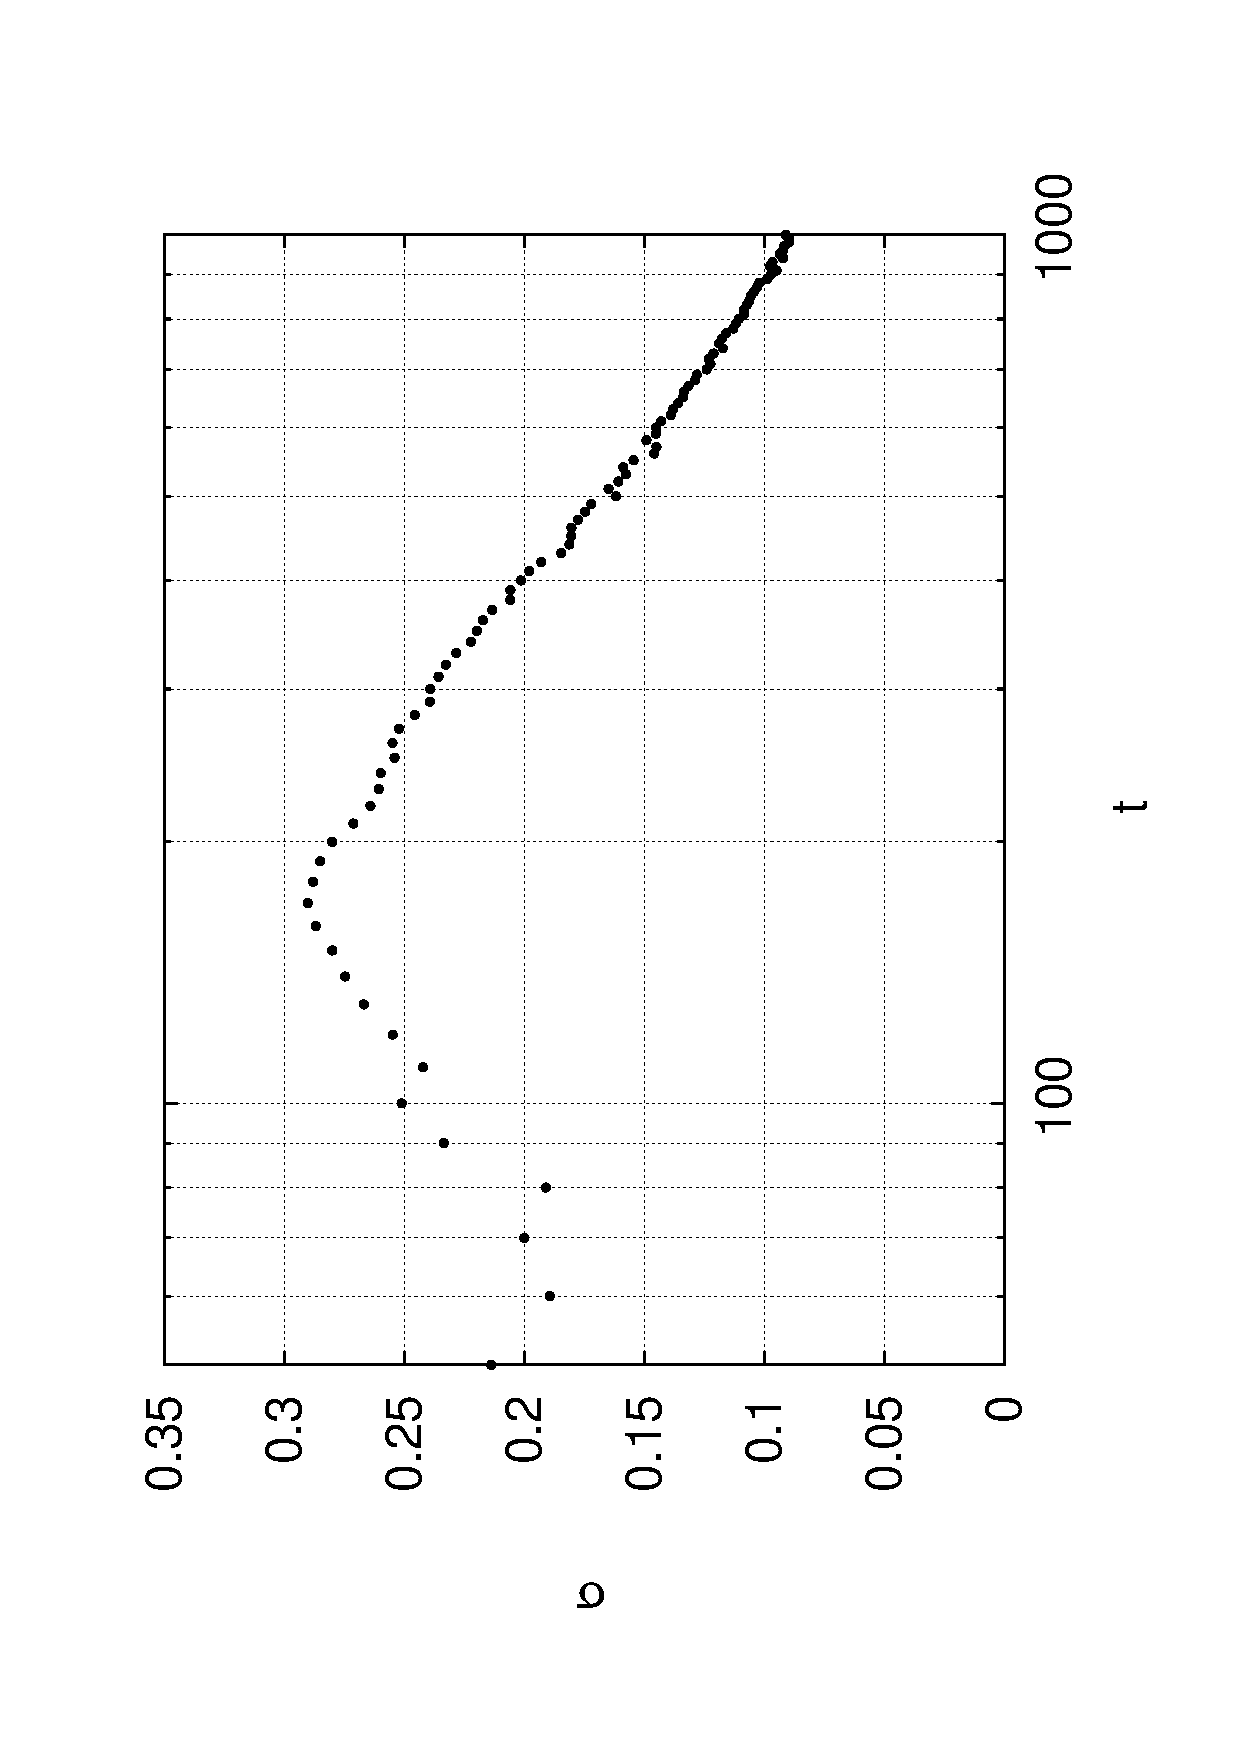
\includegraphics{test.png}
    \caption{Рисунок без метки}
    % ОШИБКА: Окружение figure должно содержать \label{}
\end{figure}

\begin{table}[h]
    \centering
    \begin{tabular}{|c|c|}
        \hline
        X & Y \\
        \hline
        3 & 4 \\
        \hline
    \end{tabular}
    \caption{Таблица без метки}
    % ОШИБКА: Окружение table должно содержать \label{}
\end{table}

\begin{lstlisting}[language=Python, caption=Код без метки]
def hello_world():
    print("Hello, World!")
# ОШИБКА: Окружение lstlisting должно содержать \label{}
\end{lstlisting}

\section{Смешанные примеры}

\begin{equation}
    \int_{0}^{\infty} e^{-x} dx = 1
    \label{eq:integral}
\end{equation}

\begin{equation}
    \sum_{n=1}^{\infty} \frac{1}{n^2} = \frac{\pi^2}{6}
    \label{eq:basel}  
\end{equation}

% Используем только одну из меток различными способами
Формула интеграла показана в~\eqref{eq:integral}.
Также можно сослаться через \cref{eq:integral}.
Автоссылка: \autoref{eq:integral}.
Ссылка на страницу: см. стр.~\pageref{eq:integral}.
% eq:basel остается неиспользованной - это ошибка!

\section{Заключение}

Этот документ демонстрирует:
\begin{itemize}
    \item Дублирующиеся метки (eq:duplicate)
    \item Ссылки на несуществующие метки (eq:nonexistent, fig:missing, eq:another_missing)
    \item Неиспользуемые метки (eq:unused_formula, tab:unused_table, eq:basel)
    \item Окружения без обязательных меток (equation, figure, table, lstlisting)
    \item Бесполезные метки в ненумерованных окружениях (eq:useless_label в equation*)
    \item Различные команды ссылок: \textbackslash ref, \textbackslash eqref, \textbackslash cref, \textbackslash autoref, \textbackslash pageref
\end{itemize}

\textbf{Поддерживаемые команды ссылок:}
\begin{itemize}
    \item Основные: \textbackslash ref, \textbackslash eqref, \textbackslash pageref
    \item Из пакета hyperref: \textbackslash autoref, \textbackslash nameref
    \item Из пакета cleveref: \textbackslash cref, \textbackslash Cref, \textbackslash cpageref
    \item Из пакета varioref: \textbackslash vref, \textbackslash vpageref
\end{itemize}

\textbf{Ожидаемые результаты проверки:}
\begin{itemize}
    \item 1 дублирующаяся метка 
    \item 3 ссылки на несуществующие метки
    \item 2 неиспользуемые метки (eq:unused_formula, tab:unused_table, но НЕ eq:basel - она используется через pageref)
    \item 4 окружения без обязательных меток
    \item 1 бесполезная метка в ненумерованном окружении
\end{itemize}

\end{document} 